\documentclass{article}

\usepackage{neurips_2026}

\usepackage[utf8]{inputenc}
\usepackage[T1]{fontenc}
\usepackage{hyperref}
\usepackage{url}
\usepackage{booktabs}
\usepackage{amsfonts}
\usepackage{amssymb}
\usepackage{amsmath}
\usepackage{nicefrac}
\usepackage{microtype}
\usepackage{xcolor}
\usepackage{graphicx}
\usepackage{array}
\usepackage{enumitem}
\usepackage{placeins}

\newcommand{\method}[1]{\texttt{#1}}

\title{Collective Semantic Memory: Merge, Trust, and Staleness for Peer Memory in Multi-Agent Navigation}

%\author{%
%  Anonymous Authors \\
%  Anonymous Institution \\
%  Anonymous Address \\
%  \texttt{anonymous@anonymous.edu} \\
%}

\begin{document}

\maketitle

\begin{abstract}
\textbf{Problem.} Collective memory is often treated as monotone: more shared information should help. In cooperative navigation with scarce semantic targets, this intuition fails. Fast global sharing improves target materialization but causes agents to race for the same targets; slow sharing avoids contention but leaves agents with stale or incomplete memories.
\textbf{Approach.} We instantiate four memory topologies over the same symbolic-semantic substrate: independent private memories, a shared event bus, a central consensus aggregator, and peer-to-peer broadcast with cadence $K$. We then introduce a minimal \emph{collective semantic memory} (CSM): peer broadcast plus explicit \emph{merge}, \emph{trust}, and \emph{staleness} rules. Q/R/M/C stage rates are used only as measurement instrumentation, not as the contribution of this paper.
\textbf{Findings.} On a 35{,}640-run multi-agent sweep, the fixed-cadence peer family exhibits a bottleneck shift: fast broadcast saturates materialization but collapses completion, while slow broadcast has the opposite profile. Mean time-to-success has an interior optimum at $K{=}8$. On a 3{,}240-run scarcity benchmark, the minimal CSM strictly dominates five fixed-cadence peer baselines on success rate: CSM reaches $0.617$ with 95\% CI $[0.610,0.624]$, above every peer-K upper CI.
\textbf{Scope.} Experiments are grid-world substrates. The claim is not that this is a complete theory of collective memory; it is a reproducible architecture split showing that merge/trust/staleness are the right explicit control surfaces after cadence alone is exhausted.
\end{abstract}

\section{Introduction}

Many multi-agent systems share information either by writing to a
single global memory, by sending learned messages, or by periodically
exchanging local state. These mechanisms are usually evaluated
end-to-end. If success improves, communication is judged useful; if it
does not, the reason is opaque. This paper studies a narrower
architectural question: when multiple agents maintain semantic memory
about places, what should be shared, at what rate, and with what
weight?

The answer is not ``share everything as soon as possible.'' In a
scarcity setting, where $N$ agents compete for $T<N$ semantic targets,
fresh global memory can make all agents select the same target. The
memory is then accurate but unhelpful. Conversely, no communication
prevents herding but starves agents of useful discoveries made by
peers. The design problem is therefore a trade-off between semantic
freshness and occupancy contention.

We make three contributions.
\begin{enumerate}[leftmargin=20pt,itemsep=2pt,topsep=2pt]
\item \textbf{Architecture split.} We implement and compare four memory topologies over the same symbolic substrate: independent, shared-bus, central-aggregator, and peer-to-peer broadcast.
\item \textbf{Cadence result.} We show that peer broadcast exposes a real coordination parameter $K$: fast broadcast improves $P(M^\star|R^\star)$ but hurts $P(C^\star|M^\star)$; the efficiency metric has an interior optimum.
\item \textbf{Minimal CSM.} We instantiate collective semantic memory with three explicit rules: merge, trust, and staleness. The minimal CSM reaches a new point on the M$\times$C plane and strictly dominates fixed-cadence peer baselines on success rate in the scarcity benchmark.
\end{enumerate}

\paragraph{Relation to the companion Q/R/M/C paper.}
The companion paper treats Q/R/M/C as a diagnostic framework. Here
those stage rates are used as measuring instruments. The main object
is different: the design of distributed symbolic memory itself.

\section{Memory substrate and task}
\label{sec:substrate}

Each agent observes a grid environment and emits semantic place
evidence such as \texttt{water\_source}, \texttt{hazard\_edge}, and
\texttt{open}. A local memory stores place records, tag confidences,
visit counts, freshness, and transition statistics. Planner queries
retrieve candidate places by matching required, preferred, and penalty
tags. A selected candidate is materialized into a concrete cell and
executed by a local controller.

The multi-agent task uses a $12{\times}10$ grid. Each agent must reach
a cell tagged \texttt{water\_source}. Targets are scarce:
$N{\in}\{3,5,8\}$ agents, $T{\le}N$ targets, three layouts, three
hazard densities, and 40 seeds for the main cadence sweep. Every run
logs Q/R/M/C events per agent:
\[
Q^\star \rightarrow R^\star \rightarrow M^\star \rightarrow C^\star,
\]
where $M^\star$ means a semantic candidate was locked as an actionable
target and $C^\star$ means the target was reached. These logs are not
the architectural contribution; they let us see where each topology
fails.

\section{Four collective-memory topologies}
\label{sec:archs}

\begin{figure}[t]
  \centering
  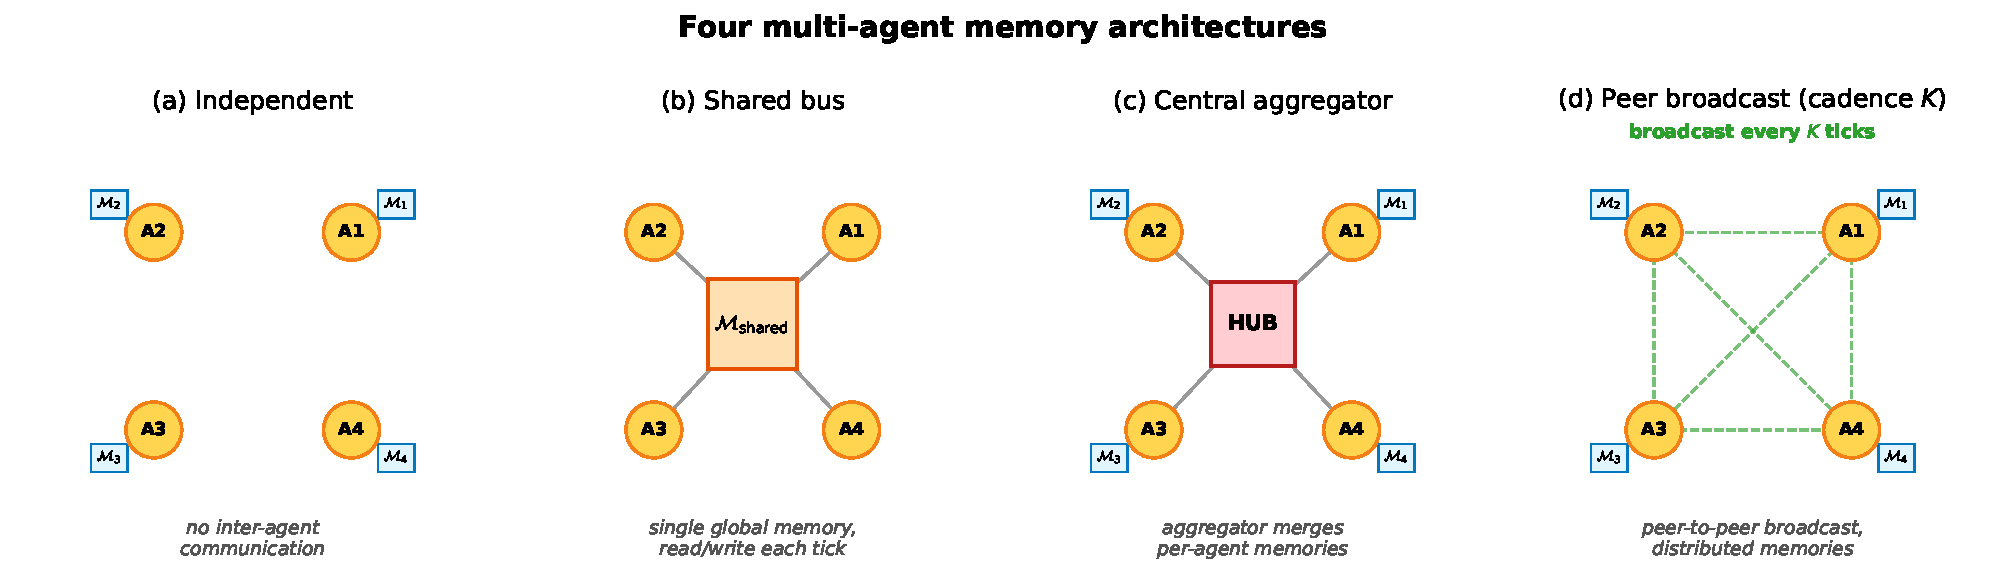
\includegraphics[width=\linewidth]{figures/fig_architectures.pdf}
  \caption{Four memory topologies. \textbf{(a)} Independent: per-agent private memory, no exchange. \textbf{(b)} Shared bus: one global memory, every agent reads and writes each tick. \textbf{(c)} Central aggregator: private memories plus a hub that merges snapshots into a consensus report. \textbf{(d)} Peer-to-peer broadcast: private memories with snapshot exchange every $K$ ticks and per-agent merged views.}
  \label{fig:architectures}
\end{figure}

The four topologies share the same local memory and planner. They
differ only in where merge happens.

\begin{description}[leftmargin=10pt,topsep=2pt,itemsep=2pt]
\item[Independent.] Each agent owns a private event store and concept graph. There is no communication path.
\item[Shared bus.] All observations are appended to a single global event bus. One shared concept graph is rebuilt from the union of all events.
\item[Central aggregator.] Each agent owns a private concept graph; a central consensus layer pulls snapshots and computes one trust-weighted report for everyone.
\item[Peer broadcast.] Each agent owns a private concept graph and a private merged view. Every $K$ ticks, agents broadcast snapshots; each agent merges its own memory with the latest snapshot from each peer.
\end{description}

The key distinction is not the clustering primitive. It is the level at
which that primitive is instantiated:
\[
\begin{array}{rcl}
\text{independent} &:& N \text{ graphs, }0\text{ mergers}\\
\text{shared bus} &:& 1 \text{ graph, }1\text{ implicit global merger}\\
\text{central} &:& N \text{ graphs }+1\text{ central merger}\\
\text{peer} &:& N \text{ graphs }+N\text{ private mergers.}
\end{array}
\]

\section{Cadence exposes the failure mode}
\label{sec:cadence}

The peer topology has one explicit parameter: broadcast cadence $K$.
The main sweep crosses four architectures and eight peer cadences
$K{\in}\{1,2,4,8,16,32,48,64\}$ for 35{,}640 runs. Figure~\ref{fig:conditional-rates}
summarizes the result.

\begin{figure}[t]
  \centering
  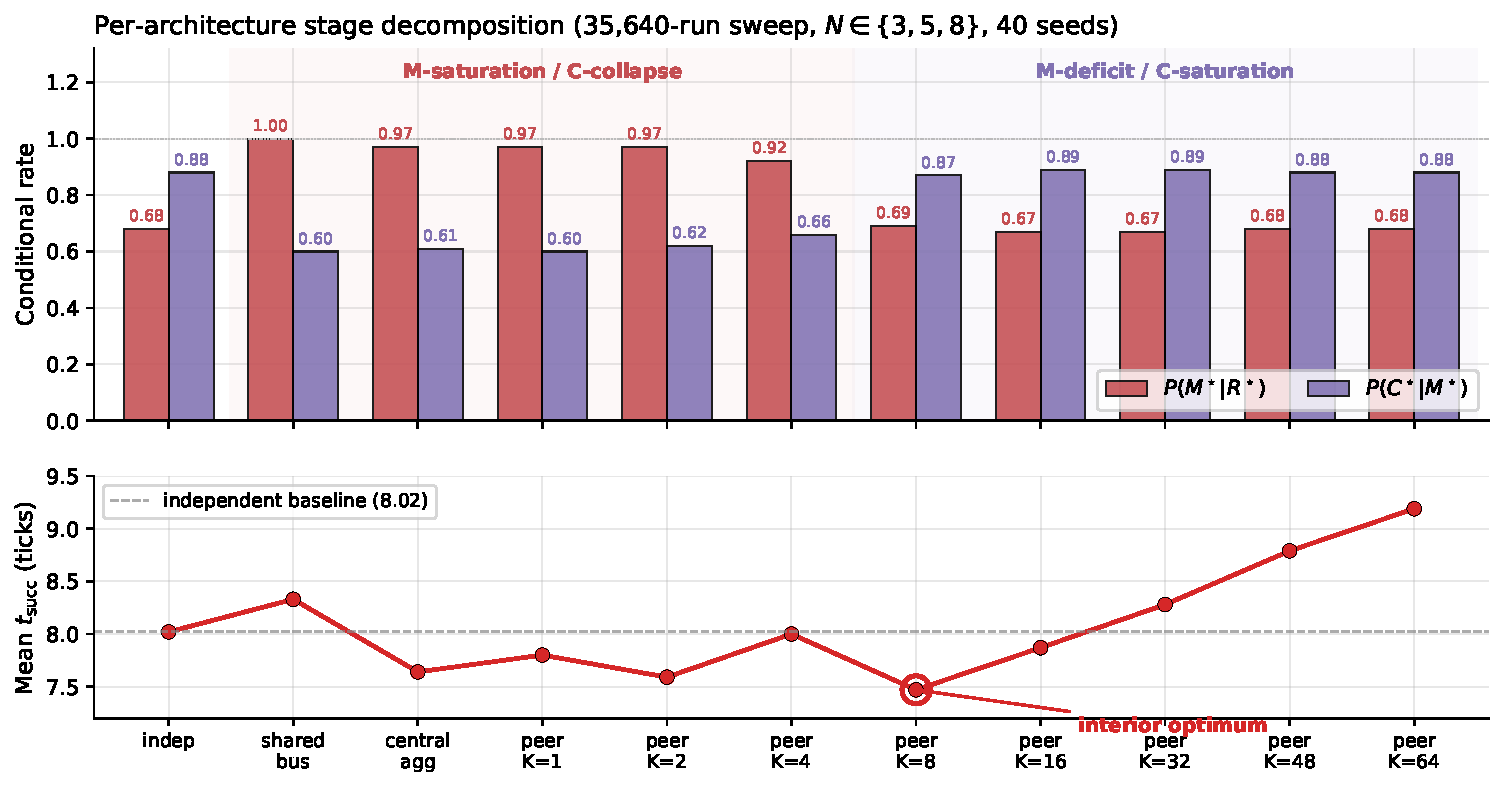
\includegraphics[width=\linewidth]{figures/fig_conditional_rates.pdf}
  \caption{Conditional rates and mean time-to-success from the 35{,}640-run sweep. Fast sharing improves target materialization but harms completion through contention; slow sharing has the opposite profile. Mean time-to-success has an interior optimum at $K{=}8$.}
  \label{fig:conditional-rates}
\end{figure}

Fast peer broadcast and centralized sharing live in the
M-saturation/C-collapse regime: agents can lock targets reliably, but
many locks point to targets that peers also pursue. Independent and
slow peer broadcast live in the M-deficit/C-saturation regime: fewer
agents lock onto good targets, but those that do are less likely to
collide with peer occupancy.

\begin{figure}[t]
  \centering
  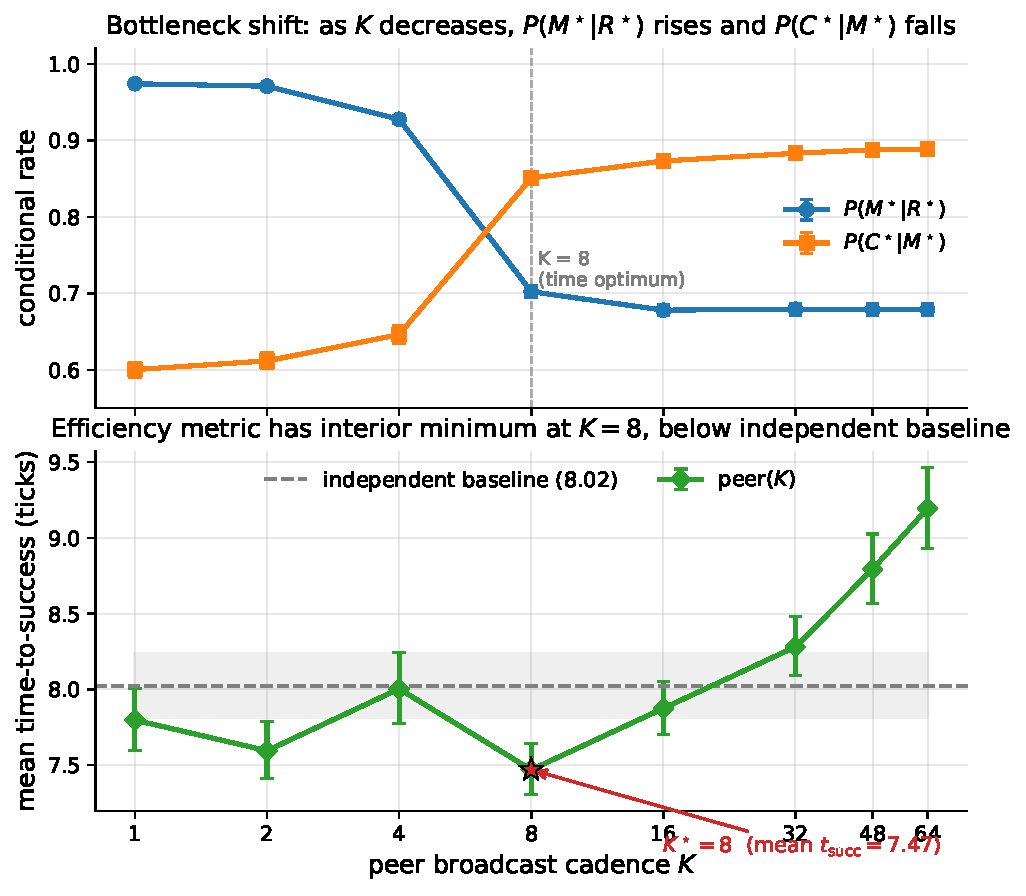
\includegraphics[width=0.85\linewidth]{figures/fig_bottleneck_shift.pdf}
  \caption{Bottleneck shift across peer cadences. $P(M^\star|R^\star)$ falls and $P(C^\star|M^\star)$ rises as $K$ grows. The practical efficiency metric, mean time-to-success, is minimized at $K{=}8$.}
  \label{fig:bottleneck-shift}
\end{figure}

Across all peer runs, Spearman of $P(M^\star|R^\star)$ vs $K$ is
$-0.608$ and of $P(C^\star|M^\star)$ vs $K$ is $+0.420$ (both
$p<10^{-4}$). The stronger signature is visible at fixed cadence:
the within-cadence Pearson correlation between the M and C links peaks
at $-0.61$ for $K{=}4$ and decays toward noise as $K$ grows. Cadence
therefore does not simply tune ``amount of communication.'' It moves
the bottleneck between semantic commitment and shared-resource
completion.

\section{Minimal collective semantic memory}
\label{sec:csm}

The cadence sweep shows that fixed-rate snapshot exchange exposes only
one control surface. A collective semantic memory should expose at
least three:
\begin{description}[leftmargin=14pt,itemsep=1pt,topsep=2pt]
\item[Merge.] How peer evidence about the same semantic place is combined.
\item[Trust.] How evidence from different peers is weighted when it conflicts or becomes unreliable.
\item[Staleness.] How old evidence decays before it influences retrieval.
\end{description}

The minimal CSM uses peer broadcast at $K{=}8$ and overlays three
rules:
\begin{description}[leftmargin=14pt,itemsep=1pt,topsep=2pt]
\item[\textit{Merge.}] Per-place score equals own evidence at weight 1 plus peer evidence at weight $\mathrm{trust}_i \cdot e^{-\alpha \cdot \mathrm{age}}$, with $\alpha=0.05$. Inclusion threshold $\tau=0.30$.
\item[\textit{Trust.}] Per-peer EMA on retrieval-success consistency. Peers whose latest snapshot supports the locally locked target gain trust; others decay toward $0.4$. Update rate $\beta=0.10$.
\item[\textit{Staleness.}] Each broadcast snapshot is timestamped; merge weight decays as $e^{-\alpha\cdot\mathrm{age}}$. Snapshots older than $10K$ ticks are pruned.
\end{description}

The implementation is a drop-in replacement for fixed-cadence peer
memory: \method{experiments/collective\_semantic\_memory/csm\_memory.py}.

\subsection{Results}

We compare CSM against fixed-cadence peer broadcast at
$K \in \{1,4,8,16,64\}$ on scarcity cells
$(N,T){\in}\{(3,2),(5,3),(8,5)\}$, three layouts, three hazard
densities, and 20 seeds: 3{,}240 runs total.

\begin{table}[ht]
\caption{Minimal CSM vs fixed-cadence peer broadcast on the scarcity benchmark. CSM's lower 95\% bootstrap CI bound exceeds every peer-K upper CI.}
\label{tab:csm-results}
\centering
\small
\begin{tabular}{l c c c}
\toprule
Architecture & $P(M^\star|R^\star)$ & $P(C^\star|M^\star)$ & Success rate (95\% CI) \\
\midrule
peer ($K{=}1$)  & 0.991 & 0.586 & 0.577 [0.572, 0.586] \\
peer ($K{=}4$)  & 0.955 & 0.623 & 0.581 [0.572, 0.590] \\
peer ($K{=}8$)  & 0.730 & 0.871 & 0.599 [0.591, 0.607] \\
peer ($K{=}16$) & 0.697 & 0.892 & 0.597 [0.589, 0.606] \\
peer ($K{=}64$) & 0.684 & 0.900 & 0.601 [0.594, 0.609] \\
\textbf{CSM (minimal)} & \textbf{0.782} & \textbf{0.825} & \textbf{0.617 [0.610, 0.624]} \\
\bottomrule
\end{tabular}
\end{table}

CSM occupies a third regime. Fast broadcasts have excellent
materialization but poor completion; slow broadcasts have the reverse.
CSM keeps both conditional links above 0.78. The absolute success gain
is modest, $+1.7$ to $+4.0$ percentage points, but the stage
decomposition shows why it is meaningful: the architecture changes the
joint M$\times$C operating point rather than merely moving along the
fixed-cadence curve.

\paragraph{Why CSM wins: the gate, not the sharing.} Provenance
annotation of the same runs gives the mechanism. CSM does not share
\emph{better} than fixed-cadence peers --- it \emph{refuses to act on
stale or untrusted foreign evidence}. The inclusion rule of
Section~\ref{sec:csm} implies a closed-form horizon beyond which a
peer's evidence can no longer form an intention,
$\mathrm{age}_{\max}(\mathrm{trust}_i) = \alpha^{-1}
\ln(\mathrm{trust}_i \cdot c/\tau)$, and this horizon is empirically
exact: measured intention-formation cutoffs match the formula
tick-for-tick across trust levels (23/23.05, 18/18.59, 12/12.84 at
$\mathrm{trust}=1.0/0.8/0.6$), including a registered-prediction
hold-out on six never-run cells ($6/6$ exact integer breakpoints) and
a discrete trust-flip: $\mathrm{trust}\le\tau/c$ zeroes
foreign-evidence commitments entirely. Fixed-cadence peers have no
such gate --- their foreign evidence never expires --- which is
precisely why their completion collapses when sharing is fast. The
full provenance-conditioned analysis appears in a companion
manuscript; here it serves as the mechanistic reading of
Table~\ref{tab:csm-results}.

\section{Place identity from meaning: removing the shared frame}
\label{sec:semantic-identity}

Everything above --- and the categorical reading below --- assumes a
shared spatial basis $X$: `the same place' means `the same $(x,y)$ in
a frame the environment hands to every agent'. This section removes
that assumption and reports what it was hiding. Each agent now holds a
\emph{private} frame (the true grid under a secret translation, and,
in the final experiment, a secret $90^\circ$-multiple rotation);
broadcast snapshots carry the sender's private coordinates, which are
meaningless to the receiver until it decides what the sender's places
\emph{mean}.

\paragraph{Mechanism.} A \emph{place fingerprint} is the local
semantic constellation around a visited cell: which content tags
(hazards, walls, water) sit at which relative offsets ---
translation-invariant and coordinate-free. Two agents match places by
\emph{mutually unique} fingerprint correspondence (each side is the
other's sole candidate; one-directional uniqueness aliases distant
look-alikes into the receiver's neighbourhood, and border-only
patterns are excluded as descriptions of the world's shape rather
than of a place). The inter-agent frame is the modal translation of
$\ge 3$ agreeing matched pairs; under rotations, one hypothesis per
$90^\circ$ reuses the same aligner and the winner must dominate the
runner-up's consensus by $2\times$. Foreign evidence --- including
places the receiver has never seen --- is then transported through
the recovered frame.

\paragraph{Results.} Registered before execution; full protocol in
the companion manuscript.
\begin{enumerate}[leftmargin=20pt,itemsep=2pt,topsep=2pt]
\item \textbf{Exact recovery.} Witness--traveler: the secret offset is
  recovered exactly in $100\%$ of landmark-world runs, and under full
  $SE(2)$ frames in $80/80$ rotation$\times$offset$\times$seed
  combinations, with $100\%$ completion on foreign-committed locks.
\item \textbf{Failure asymmetry.} Where identification is impossible
  --- a featureless region, or a $180^\circ$-symmetric layout in which
  the frame is unrecoverable \emph{in principle} --- semantic identity
  makes \emph{zero} commitments (fails closed), while coordinate
  identity keeps confidently locking wrong cells ($100\%$ wrong locks;
  fails open).
\item \textbf{The full stack.} With $N{=}4$ agents in distinct secret
  frames, alignment develops online (onset in $100\%$ of episodes,
  mean tick ${\approx}15$) and recovers $88\%$ of the shared-frame
  performance gap (success $0.444$ vs.\ $0.456$ oracle vs.\ $0.350$
  coordinate); under random $SE(2)$ frames every semantic commitment
  points at real water ($8/8$) while the coordinate stack produces
  $992$ phantom locks ($0$ real).
\item \textbf{The gate is orthogonal.} Re-running the
  $\mathrm{age}_{\max}$ analysis above with the CSM inclusion rule ON
  TOP of semantic identity, under a frame offset and under a
  $90^\circ$ rotation, reproduces the SAME integer breakpoints
  ($20/14/9$; $\mathrm{bp}=20$ rotated) --- the trust$\times$staleness
  gate and frame recovery are independent layers.
\end{enumerate}

The stronger claim promised in earlier drafts' limitations is
therefore discharged constructively: place identity can be carried by
meaning alone, it composes with merge/trust/staleness unchanged, and
--- unlike the coordinate convention it replaces --- it knows when it
does not know.

\paragraph{The categorical indicator: adjunction round-trip defect.}
Frame recovery is exactly the operation the categorical reading of
\S\ref{sec:categorical} needs once the shared basis $X$ is dropped: with
private frames each agent carries its own place category, and
communication is a pair of recovery functors $F=\textsc{align}(A,B)$
(the sender $B$'s frame expressed in receiver $A$'s coordinates) and
$G=\textsc{align}(B,A)$. If the two are genuinely adjoint --- the frames
are glued --- the round trip $\eta_X: X\to G(F(X))$ is the identity, so
the \emph{adjunction defect}
\[
\mathrm{def}=\lVert F.\mathrm{offset}+G.\mathrm{offset}\rVert_1
\ \text{(translation)},\qquad
r_F{+}r_G\equiv 0\,(\mathrm{mod}\,4)\ \text{and}\
\lVert R_{r_G}F.\delta+G.\delta\rVert_1\ (SE(2)),
\]
is zero \citep{maclane1998categories}. Measured on the recovery method
above (\texttt{experiments/warp/alignment\_defect.py}, 3 offsets
$\times$ 10 seeds per cell): the defect is \emph{exactly} $0$ in $30/30$
runs for translation frames and $30/30$ for each of the four $90^\circ$
rotations --- the recovered functors are strict adjoints. Where recovery
must fail (an agent that has observed only a featureless interior band),
$F$ or $G$ is undefined in $30/30$ runs with \emph{zero} spurious
gluings ($\mathrm{def}>0$): no adjoint exists and the aligner refuses to
build one. The exact discrete aligner therefore realizes a dichotomy ---
strict adjoint ($\mathrm{def}{=}0$) or no adjunction --- and never a
confident wrong gluing; ``failing closed'' above is precisely
\emph{refusing a non-adjoint pair}. This is the quantity the categorical
model computes that a re-description does not: a scalar that is zero iff
the collective's local frames are coherently glued, and it is this
gluing --- not a shared coordinate convention --- that
\S\ref{sec:categorical}'s merge silently presupposed.

\section{Categorical BDI reading of collective semantic memory}
\label{sec:categorical}

This section gives a compact theoretical reading of the water-search
example in terms of belief, desire, and intention. The goal is not to
introduce a new planner, but to make explicit the mathematical
structure already used by the collective semantic memory architecture.

We assume a finite set of agents $A=\{1,\ldots,N\}$, a shared spatial
basis $X$, and a shared semantic alphabet $\Sigma$. In the present
grid-world implementation, $X$ is the common coordinate frame and
$\Sigma$ contains tags such as \texttt{water\_source},
\texttt{water\_candidate}, \texttt{hazard\_edge}, and \texttt{open}.
This is an explicit modelling assumption. The agents may have different
observations, different memories, and different confidence values, but
they interpret places in a common coordinate framework and express
semantic evidence in a common tag alphabet. Without the first
assumption, peer merge requires a place-alignment problem to be solved
first --- Section~\ref{sec:semantic-identity} solves it constructively
(fingerprint consensus recovers the inter-agent frame), and
Section~\ref{sec:colimit} states what that construction is,
categorically. Symbol alignment (a shared $\Sigma$) remains assumed.

At time $t$, agent $i$ maintains a local semantic context
$\mathcal{K}_t^i=(G_t^i,\Sigma,I_t^i)$, where $G_t^i$ is the set of
place records stored in the agent's private memory, and
\[
I_t^i \subseteq G_t^i \times \Sigma
\]
is the thresholded incidence relation saying that place $g\in G_t^i$
carries tag $\sigma\in\Sigma$ with sufficient confidence. The graded
implementation uses tag confidences and weighted scores; the crisp
relation $I_t^i$ is the thresholded skeleton needed for the theoretical
description.

This formal context induces a Galois connection between sets of tags
and sets of places:
\[
\operatorname{ext}_t^i(B)=\{g\in G_t^i:\forall\sigma\in B,\ (g,\sigma)\in I_t^i\},
\qquad
\operatorname{int}_t^i(S)=\{\sigma\in\Sigma:\forall g\in S,\ (g,\sigma)\in I_t^i\}.
\]
For a water-search task, the desired semantic predicate is
$B_{\mathrm{water}}=\{\texttt{water\_source}\}$, or, in the implemented
weighted form, a predicate combining positive evidence for
\texttt{water\_source}, \texttt{water\_candidate}, and
\texttt{water\_nearby} with penalties for \texttt{hazard\_edge} or
nearby risk. Retrieval succeeds for agent $i$ at time $t$ exactly when
\[
\operatorname{ext}_t^i(B_{\mathrm{water}})\neq\varnothing .
\]
Thus the retrieval stage is not a coordinate lookup. It is the test
that the queried semantic meaning already has a non-empty extent in the
agent's realized memory.

We can now define the BDI components.

\paragraph{Belief.} The belief state of agent $i$ is the structured
semantic memory induced by $\mathcal{K}_t^i$. Equivalently, it is the
concept lattice $L_t^i=\operatorname{Concepts}(\mathcal{K}_t^i)$, whose
nodes pair extents of places with intensions of tags. A water belief is
not the proposition ``there is water at coordinate $x$.'' It is the
region of $L_t^i$ whose intension contains the water predicate. If this
region is empty, the agent does not merely choose badly; the relevant
semantic object is absent from its current memory.

\paragraph{Desire.} Desire is a state-conditioned semantic predicate
over the belief lattice. In the water example, the agent's internal
state contains a thirst variable. The active desire can be written as
\[
D_t^i =
\begin{cases}
B_{\mathrm{water}}, & \text{if } \mathrm{thirst}_t^i\geq\theta_{\mathrm{on}},\\
B_{\mathrm{goal}}, & \text{otherwise.}
\end{cases}
\]
Thus desire is not an additional metaphysical object. It is the rule
that selects which semantic predicate should be queried from the
current belief structure.

\paragraph{Intention.} Intention is the commitment to one materialized
candidate. Once desire has selected a predicate and retrieval has
produced a non-empty extent, the planner applies a satisficing choice
function
\[
\chi_t^i:\mathcal{P}(G_t^i)\rightarrow G_t^i\cup\{\bot\},
\qquad
g_t^{i,\star}=\chi_t^i\!\big(\operatorname{ext}_t^i(D_t^i)\big),
\]
where $\bot$ denotes failure to materialize a target. In Q/R/M/C terms,
desire determines the query $Q^\star$, belief supports retrieval
$R^\star$, and intention corresponds to materialization $M^\star$.
Completion $C^\star$ is downstream of this semantic structure: it
depends on whether the physical controller reaches the locked target
and whether the target remains available under multi-agent occupancy.

This gives a compact categorical reading. Let $\mathbf{Ctx}_\Sigma$ be
the category whose objects are semantic contexts $(G,\Sigma,I)$ over the
fixed alphabet $\Sigma$, and whose morphisms preserve semantic
incidence. A local memory trajectory for agent $i$ is a time-indexed
diagram
\[
\mathcal{K}_0^i\rightarrow\mathcal{K}_1^i\rightarrow\cdots
\rightarrow\mathcal{K}_t^i\rightarrow\mathcal{K}_{t+1}^i\rightarrow\cdots
\]
in $\mathbf{Ctx}_\Sigma$. Each arrow is induced by observation and
memory update. When new evidence is consolidated, the formal context
changes; therefore its concept lattice changes. This is the
order-theoretic content of memory growth.

In Q/R/M/C terms, an empty extent
$\operatorname{ext}_t^i(D_t^i)=\varnothing$ is a belief/retrieval
failure, a non-empty extent with no stable lock is a materialization
failure, and a successful lock that cannot be reached is a completion
failure --- the semantic and the physical parts of the agent's state
fail in different, separately measurable ways.

The collective case lifts this by one construction. At broadcast times
the receiver $i$ holds a diagram of local memory objects
$\mathcal{D}_t^i=(\mathcal{K}_t^i,\mathcal{K}_t^{j_1},\ldots,
\mathcal{K}_t^{j_m})$ together with alignment maps, and queries the
merged consensus object
$\widetilde{\mathcal{K}}_t^i=\operatorname{Merge}_{\mathrm{trust},
\mathrm{stale}}(\mathcal{D}_t^i)$, with peer evidence weighted exactly
by the rules of Section~\ref{sec:csm}
($\mathrm{trust}_{j\to i}\cdot e^{-\alpha\,\mathrm{age}_j}$). The same
BDI definitions apply to the merged context: intention is now selected
from $\operatorname{ext}_{\widetilde{\mathcal{K}}_t^i}(D_t^i)$ rather
than from the private extent alone.

This explains why communication cadence produces a bottleneck shift.
Faster broadcast increases the freshness of peer evidence. This tends
to enlarge or improve the water extent
$\operatorname{ext}_{\widetilde{\mathcal{K}}_t^i}(B_{\mathrm{water}})$,
so agents can materialize targets more reliably; in Q/R/M/C terms, this
raises $P(M^\star\mid R^\star)$. But the same fresh shared belief also
synchronizes intentions. Several agents may lock onto the same scarce
water source. The memory is semantically accurate, but the physical
target is now contested. This lowers $P(C^\star\mid M^\star)$. The
bottleneck is therefore physically grounded. It is not a formal
artifact of the decomposition: it arises because semantic belief is
shared through memory, while completion is constrained by occupancy and
scarce resources. Collective semantic memory must therefore regulate
not only how much information is shared, but also how it is merged,
whose evidence is trusted, and when stale evidence should stop
influencing intention formation.

In this sense the ``collective'' is not a central mind and not a global
map but a stabilised family of peer-indexed processes; the next
subsection makes that statement precise.

The dual, process-level reading --- agents as coalgebras (codata), the
collective as a final coalgebra, communication as depth-one
corecursion, and the bottleneck shift as a competition between belief-
and intention-bisimilarity --- is developed in
Appendix~\ref{sec:coalgebra}. It is a lens, not a mechanism: nothing
downstream depends on it, which is why it lives in the appendix.

\subsection{Colimit merge and its invariants}
\label{sec:colimit}

The merge object above can be described more precisely. Working in a
timestamp- and provenance-enriched version of $\mathbf{Ctx}_\Sigma$, a
snapshot merge from agents $1,\dots,N$ is a diagram of local memory
objects plus alignment maps induced by the place-identity relation. The
consensus object $\widetilde{\mathcal{K}}_t^i$ is the colimit of this
diagram, implemented concretely by the union-find merge over aligned
concepts. This reading gives three useful constraints.
\begin{enumerate}[leftmargin=20pt,itemsep=2pt,topsep=2pt]
\item \textbf{Order independence.} The merged object is unique up to isomorphism, so the result is not an artefact of processing agent snapshots in a particular order.
\item \textbf{Chaining is expected.} If concept A aligns with B and B aligns with C, union-find performs the transitive closure. Over-merging is therefore not a bug in the data structure; it is the cost of the chosen equivalence relation.
\item \textbf{Decay is not a morphism.} Staleness is kept as a weight field outside the alignment morphisms. Otherwise age-then-merge and merge-then-age need not commute, breaking the clean interpretation of broadcast snapshots as one diagram.
\end{enumerate}

In earlier drafts this section ended by conceding that the model does
not answer which perceptual features should identify two places ---
the alignment maps were assumed, not constructed. That gap is now
closed by Section~\ref{sec:semantic-identity}, and the closure gives
the colimit reading its missing scientific function:
\begin{enumerate}[leftmargin=20pt,itemsep=2pt,topsep=2pt]
\item \textbf{The alignment morphisms are constructed, not assumed.}
  Fingerprint consensus IS an algorithm that produces the alignment
  maps of the diagram --- mutually-unique landmark matches determine
  the frame transform through which every local memory object embeds.
\item \textbf{Existence becomes an empirical predicate.} The colimit
  exists iff the consensus does. In a $180^\circ$-symmetric world the
  alignment morphism does not exist \emph{in principle} (two
  incomparable diagrams support equal consensus), and the
  implementation detects exactly this and refuses to merge --- the
  fail-closed behaviour of Section~\ref{sec:semantic-identity} is the
  categorical non-existence made operational. This predicate is
  measured, not asserted: the adjunction round-trip defect of
  \S\ref{sec:semantic-identity} is exactly $0$ when the pairwise
  alignment is a strict adjoint (in every recovered translation and
  $90^\circ$-rotation case, $30/30$) and undefined when no adjoint
  exists (fail-closed, $30/30$, with zero spurious gluings) --- a scalar
  witness for colimit existence.
\item \textbf{Decay stays outside the morphisms} (invariant 3), and
  empirically the trust$\times$staleness gate is unchanged by frame
  recovery --- the same integer breakpoints with and without a shared
  frame --- confirming that the two layers commute as the diagram
  reading requires.
\end{enumerate}

\section{Limitations and next experiments}
\label{sec:limitations}

\textbf{Grid substrate.} The current result is intentionally controlled:
all experiments are in grid worlds. A continuous-state substrate such
as VMAS, Habitat, ProcTHOR, or MiniWorld is the next portability step.

\textbf{Coordinate anchor.} Removed in
Section~\ref{sec:semantic-identity}: local fingerprint signatures
recover the inter-agent frame (translation and $90^\circ$ rotations)
exactly, and the merge/trust/staleness results are unchanged on top of
the recovered frames. What remains open is the harder end of the same
axis: continuous $SE(2)$, appearance noise (the current matcher uses
exact constellation equality because the substrate is noise-free), and
symbol alignment --- agents with \emph{different tag alphabets} still
cannot merge.

\textbf{Minimal CSM.} The CSM rules are deliberately simple. Adaptive
cadence $K_t$, intent-conditioned trust, and selective consolidation of
under-represented tags are the next architecture variants.

\textbf{Learned baselines.} CommNet-style learned communication is a
useful comparison, but the more relevant future baseline is an explicit
memory LLM or vector-memory multi-agent system measured on the same
task.

\section{Conclusion}

Collective memory is not monotone. In scarce multi-agent navigation,
instant information sharing can reduce completion by causing agents to
converge on the same targets. Peer cadence exposes the trade-off, but
cadence alone is a one-dimensional control surface. A collective
semantic memory should make merge, trust, and staleness explicit. The
minimal CSM does exactly that and moves the system to a new operating
point: neither fast-broadcast M-saturation nor slow-broadcast
C-saturation, but a more balanced M$\times$C profile with higher
success than every fixed peer cadence in the scarcity benchmark.

\begin{ack}
This manuscript is prepared in anonymized form for review. The
reported experiments were run from the same benchmark pipeline as the
companion Q/R/M/C measurement paper, but the architectural claim here
is restricted to collective semantic memory.
\end{ack}

{\small
\begin{thebibliography}{9}

\bibitem[Aczel(1988)]{aczel1988nonwellfounded}
P.~Aczel.
\newblock \emph{Non-Well-Founded Sets}.
\newblock CSLI Lecture Notes 14, 1988.

\bibitem[Bettini et~al.(2022)]{bettini2022vmas}
M.~Bettini, R.~Kortvelesy, J.~Blumenkamp, and A.~Prorok.
\newblock VMAS: A vectorized multi-agent simulator for collective robot learning.
\newblock In \emph{16th International Symposium on Distributed Autonomous Robotic Systems (DARS)}, 2022.
\newblock arXiv:2207.03530.

\bibitem[Boyd et~al.(2006)]{boyd2006gossip}
S.~Boyd, A.~Ghosh, B.~Prabhakar, and D.~Shah.
\newblock Randomized gossip algorithms.
\newblock \emph{IEEE Trans.\ Information Theory}, 52(6):2508--2530, 2006.

\bibitem[Chevalier-Boisvert et~al.(2023)]{MinigridMiniworld23}
M.~Chevalier-Boisvert, B.~Lahlou, S.~Willems, and P.~S. Castro.
\newblock MiniGrid and MiniWorld: Modular reinforcement learning environments.
\newblock \emph{arXiv:2306.13831}, 2023.

\bibitem[Deitke et~al.(2022)]{deitke2022procthor}
M.~Deitke, E.~V. Wijmans, D.~Schwenk, O.~Salvador, K.~M. Ehsani, et al.
\newblock ProcTHOR: Large-scale embodied AI using procedural generation.
\newblock In \emph{NeurIPS Datasets and Benchmarks}, 2022.

\bibitem[Foerster et~al.(2018)]{foerster2018ctde}
J.~N. Foerster, G.~Farquhar, T.~Afouras, N.~Nardelli, and S.~Whiteson.
\newblock Counterfactual multi-agent policy gradients.
\newblock In \emph{AAAI}, 2018.

\bibitem[Jacobs(2016)]{jacobs2016coalgebra}
B.~Jacobs.
\newblock \emph{Introduction to Coalgebra: Towards Mathematics of States and Observation}.
\newblock Cambridge University Press, 2016.

\bibitem[Mac~Lane(1998)]{maclane1998categories}
S.~Mac~Lane.
\newblock \emph{Categories for the Working Mathematician}.
\newblock Springer, 2nd edition, 1998.

\bibitem[Rao and Georgeff(1995)]{rao1995bdi}
A.~S. Rao and M.~P. Georgeff.
\newblock BDI agents: From theory to practice.
\newblock In \emph{ICMAS}, 1995.

\bibitem[Rutten(2000)]{rutten2000universal}
J.~J.~M.~M. Rutten.
\newblock Universal coalgebra: a theory of systems.
\newblock \emph{Theoretical Computer Science}, 249(1):3--80, 2000.

\bibitem[Sangiorgi(2011)]{sangiorgi2011bisimulation}
D.~Sangiorgi.
\newblock \emph{Introduction to Bisimulation and Coinduction}.
\newblock Cambridge University Press, 2011.

\bibitem[Savva et~al.(2019)]{savva2019habitat}
M.~Savva, A.~Kadian, O.~Maksymets, Y.~Zhao, E.~Wijmans, B.~Jain, J.~Straub, J.~Liu, V.~Koltun, J.~Malik, et al.
\newblock Habitat: A platform for embodied AI research.
\newblock In \emph{ICCV}, 2019.

\bibitem[Sperber and Wilson(1995)]{sperber1995relevance}
D.~Sperber and D.~Wilson.
\newblock \emph{Relevance: Communication and Cognition}.
\newblock Blackwell, 2nd edition, 1995.

\bibitem[Sukhbaatar et~al.(2016)]{sukhbaatar2016commnet}
S.~Sukhbaatar, A.~Szlam, and R.~Fergus.
\newblock Learning multiagent communication with backpropagation.
\newblock In \emph{NeurIPS}, 2016.

\bibitem[Xiao et~al.(2007)]{xiao2007distributed}
L.~Xiao, S.~Boyd, and S.~Lall.
\newblock A scheme for robust distributed sensor fusion based on average consensus.
\newblock \emph{IPSN}, 2007.

\end{thebibliography}
}

\appendix

\section{The coalgebraic layer: individuals as codata, the collective as a final coalgebra}
\label{sec:coalgebra}

The reading of \S\ref{sec:categorical} fixes belief \emph{content}: at a
state, the concept lattice $L_t^i=\operatorname{Concepts}(\mathcal{K}_t^i)$
says what is retrievable, and the merge of \S\ref{sec:colimit} says how peer
contents combine into $\widetilde{\mathcal K}_t^i$. Both are
\emph{algebraic}: they build a belief object. Neither speaks to the agent as
a non-terminating \emph{process} that must emit an action and a signal at
every tick under a moving environment, nor to the sense in which a
\emph{population} comes to share a convention. That process side is
\emph{coalgebraic}~\citep{rutten2000universal,jacobs2016coalgebra}. We make it precise on the water-search example and show
the two sides are dual, meeting inside a single state transition. (The
belief/desire/intention vocabulary follows the BDI agent tradition
\citep{rao1995bdi}, here given coalgebraic content.)

\paragraph{Signature.} Fix an action set $\mathrm{Act}$ (move, dig, noop), a
per-agent observation set $O_i$ (agent $i$'s local percept --- its
\emph{unique view}), and an \emph{ostension} set
\[
  M \;=\; 1 \,+\, (X\times\Sigma),
\]
whose values are either \emph{silence} (the summand $1$) or a pointer
``place $x$ carries tag $\sigma$'' (whistle-and-point at a water-marked
cell). That silence is a first-class value of $M$ matters: the ostension
channel \emph{can be informatively empty}, and it is separate from the state
update below. This is exactly the observability that a learned real-valued
message vector destroys (its channel is never empty and never separates
signalling from stepping), and it is why the symbolic stages remain
readable.

\paragraph{State.} We take the coalgebra carrier to be the H-MDP high-level
state of \S\ref{sec:categorical},
\[
  \mathcal{S}_i \;=\; \big\{\, h=(\mathcal{K}^i,\,D^i,\,g^{i,\star},\,s^i) \,\big\},
\]
carrying the same information as $(L^i,D^i,g^{i,\star},s^i)$ since
$L^i=\operatorname{Concepts}(\mathcal K^i)$. Thus \emph{belief lives in the
state}; the lattice is a projection of it.

\paragraph{Definition (codata: the agent's cotype).}
The observable behaviour of agent $i$ is a coalgebra for the endofunctor
\[
  B_i(S)\;=\;\underbrace{\mathrm{Act}}_{\text{act now}}\;\times\;
            \underbrace{M}_{\text{signal now}}\;\times\;
            \underbrace{S^{\,O_i\times M^{A\setminus\{i\}}}}_{\text{continue given (my next percept, peers' signals)}},
\]
i.e. a map $c_i=\big\langle\, \method{observe\_act}_i,\ \method{observe\_ostension}_i,\ \method{step\_intension}_i \,\big\rangle : \mathcal{S}_i \to B_i(\mathcal{S}_i)$ with three destructors
\[
  \method{observe\_act}_i:\mathcal{S}_i\to\mathrm{Act},\quad
  \method{observe\_ostension}_i:\mathcal{S}_i\to M,\quad
  \method{step\_intension}_i:\mathcal{S}_i\to \mathcal{S}_i^{\,O_i\times M^{A\setminus\{i\}}} .
\]
Here $M^{A\setminus\{i\}}=\prod_{j\neq i}M$ is the tuple of peers' ostensions
delivered this tick. Operationally, $\method{step\_intension}_i(h)(o,(m_j)_{j\neq i})$
(i)~folds the percept $o$ and the peer pointers $(m_j)$ into the context by
the trust/staleness merge, $\widetilde{\mathcal K}_t^i=\operatorname{Merge}_{\mathrm{trust,stale}}(\cdots)$
of \S\ref{sec:colimit}; (ii)~recomputes the lattice; (iii)~re-evaluates the
desire predicate $D^i$; and (iv)~re-locks the intention
$g^{i,\star}=\chi_t^i(\operatorname{ext}(D^i))$ of \S\ref{sec:categorical}.
So $\operatorname{Merge}$ and $\chi$ are \emph{components of one destructor}.
The agent \emph{is} the codata generated by $c_i$: it has no finite terminal
plan, only the standing ability to emit an action and an ostension and to
continue. This is the ``infinite survival generator'' of the motivating
example.

\paragraph{Definition (indexed family).}
The system is the $A$-indexed family $\{(\mathcal{S}_i,c_i)\}_{i\in A}$, a
coalgebra in $\mathbf{Set}^{A}$. The functor $B_i$ depends on the index $i$
through $O_i$ (and through the peer set $A\setminus\{i\}$): the same survival
cotype is instantiated at each agent through that agent's local viewpoint.
Agent~1 on the dune generates from ``I see the horizon''; agent~2 in the
hollow generates from ``I feel the soil.'' The index is the viewpoint.

\paragraph{Definition (codependence: the collective coalgebra).}
Let the environment deliver a joint percept $o=(o_i)_{i\in A}\in\prod_i O_i$.
The collective one-tick map on $\prod_i\mathcal{S}_i$ wires each agent's
ostension output into the others' step inputs,
\[
  \Phi\big((h_i)_i\big)(o)\;=\;
  \Big(\ \method{step\_intension}_i(h_i)\big(o_i,\,(\method{observe\_ostension}_j(h_j))_{j\neq i}\big)\ \Big)_{i\in A}.
\]
Because $i$'s next state is a function of the \emph{destructor outputs} of
the others, the family is not $N$ independent processes but one coalgebra for
the product functor $\mathbf{B}(S)=\big(\prod_i(\mathrm{Act}\times M)\big)\times S^{\prod_i O_i}$
on $\prod_i\mathcal{S}_i$. This wiring is the \emph{codependence}: agent~1
cannot step without passing agent~2's ostension through its own
$\method{step\_intension}$. Broadcast cadence enters here as a gate: at
non-broadcast ticks the delivered tuple $(m_j)$ is the last received (stale)
tuple, or silence; $K$ is the delivery period.

\paragraph{Definition (behaviour and bisimulation).}
$B_i$ is a container (polynomial) functor, so it has a final coalgebra
$(\nu B_i,\ \mathrm{beh}_i)$~\citep{aczel1988nonwellfounded,rutten2000universal} whose elements are the $\big(O_i\times M^{A\setminus\{i\}}\big)$-branching,
$(\mathrm{Act}\times M)$-labelled behaviour trees, and there is a unique
coalgebra morphism $!_i:\mathcal{S}_i\to\nu B_i$ sending a state to its whole
future behaviour. A \emph{$B_i$-bisimulation} is a relation
$R\subseteq\mathcal{S}_i\times\mathcal{S}_i$ under which related states emit
equal action and equal ostension and, on every input, step to $R$-related
states. Container functors preserve weak pullbacks, so the \emph{greatest
bisimulation} $\sim_i$ exists, is an equivalence, and equals $\ker(!_i)$:
two states are bisimilar iff they have the same behaviour~\citep{sangiorgi2011bisimulation}. The same holds for
the collective coalgebra $(\prod_i\mathcal{S}_i,\ \langle(\method{observe\_act}_i)_i,(\method{observe\_ostension}_i)_i,\Phi\rangle)$,
with greatest bisimulation $\approx$.

\paragraph{Definition (society / culture).}
The \emph{collective} is the image of the states in the final coalgebra
$\nu\mathbf{B}$, equivalently the quotient $\big(\prod_i\mathcal{S}_i\big)/\!\approx$.
It is neither a central server nor a shared map: it is a bisimilarity class of
joint behaviour. A \emph{water-search convention} is this invariant read on
the water sub-signature. Let $M_{\mathrm{water}}\subseteq M$ be the pointers
whose tag lies in the water family, and let
$\nu B_i\to\nu B^{\mathrm{w}}$ be the forgetful map to the behaviour trees
restricted to receiving $M_{\mathrm{water}}$ and emitting the corresponding
intention lock. The population \emph{holds the convention} when all agents'
reachable behaviours agree under this map: hearing ``point-and-dig at a
water-marked place'' drives every agent's intention destructor to lock that
place (up to occupancy). Governance is then automatic in both directions. A
new agent (the example's fourth agent) is a member of the society exactly
when its behaviour lands in the class $[\cdot]_{\approx}$ on
$M_{\mathrm{water}}$ --- otherwise its ostensions are not understood and its
own step never converges (top-down); and the class itself was reached by the
local, coupled steps of the first agents at one green shrub (bottom-up).

\paragraph{Remark (communication = lazy, depth-one corecursion).}
The behaviour $!_i(h)$ is defined by unfolding $c_i$ indefinitely. On
receiving $m_j=\method{observe\_ostension}_j(h_j)$, agent $i$ uses only this
\emph{depth-one} destructor output inside $\method{step\_intension}_i$; it
does \emph{not} compute $!_j(h_j)\in\nu B_j$, the peer's full behaviour, which
is the ``I~think that you~think\ldots'' regress. Communication is therefore
corecursion truncated to the least depth that resolves the receiver's own
next step --- a finite approximation of the final-coalgebra map --- with a
relevance-theoretic stopping rule \citep{sperber1995relevance} deciding that depth. The
regress collapses into one effective action.

\paragraph{Remark (algebra--coalgebra bridge to \S\ref{sec:categorical}--\ref{sec:colimit}).}
Belief is algebraic: the FCA lattice $L_t^i$ built by the colimit merge is
the \emph{content at a state}. The agent is coalgebraic: the codata observed
by the three destructors is the \emph{process over states}. They are dual and
meet in one place --- the colimit merge and the satisficing choice $\chi$ are
the internals of $\method{step\_intension}$. The memory-growth diagram
$\mathcal{K}_0^i\to\mathcal{K}_1^i\to\cdots$ of \S\ref{sec:categorical} is
precisely the belief-projection of the coalgebra trajectory
$h_0^i\mapsto h_1^i\mapsto\cdots$.

\paragraph{Coalgebraic reading of the bottleneck shift.}
The result of \S\ref{sec:cadence} and Table~\ref{tab:csm-results} has a
one-line reading here. Two kinds of bisimilarity compete. Bisimilarity on the
\emph{ostension / belief} sub-signature is the wanted invariant: it is the
shared water convention. Bisimilarity on the raw \emph{intention} output over
a \emph{scarce} target is the unwanted one: several states mapping to the same
$g^{\star}$ is a collision. Occupancy $\mathcal{O}_{-i}$ is the
extra-coalgebraic constraint that penalises the second. Cadence $K$ tunes how
hard the coupling $\Phi$ drives the collective toward the \emph{full}
greatest bisimulation $\approx$: small $K$ delivers fresh ostensions often,
enlarging the merged water extent so intention locks reliably
($P(M^\star\mid R^\star)\uparrow$), but over-synchronises the intention
destructor so agents collide ($P(C^\star\mid M^\star)\downarrow$). The
interior optimum $K{=}8$ is where belief converges without intention
collapsing onto one cell; the minimal CSM adds trust and staleness precisely
so that $\method{step\_intension}$ reaches belief-bisimilarity (fresh,
trusted, aligned evidence) while damping intention-bisimilarity (stale
evidence decays before it can herd every agent onto the same lock). We state
this as a reading consistent with the data, not as a theorem: the container
functors, their final coalgebras, and bisimulation are standard constructions
used here as a lens, and the relevance-theoretic stopping rule is an
interpretive gloss rather than a fitted mechanism.

\begin{table}[t]
\caption{The motivating example's terms as formal objects of the coalgebraic
reading. Each row is the water-search meaning of a construction already used
in \S\ref{sec:coalgebra}.}
\label{tab:coalg-dictionary}
\centering
\small
\begin{tabular}{p{2.9cm} p{4.3cm} p{4.4cm}}
\toprule
Informal term & Formal object & Water-search meaning \\
\midrule
Cotype (codata) & $B_i$-coalgebra $(\mathcal{S}_i,c_i)$ & the agent's non-terminating action/signal generator \\
Indexed type & family over $A$; dependence of $B_i$ on $O_i$ & the agent's unique local viewpoint (dune vs.\ hollow) \\
Codependent type & wiring $\method{observe\_ostension}_j\!\to\!\method{step\_intension}_i$ in $\Phi$ & ``I step only through your ostension'' \\
Individual (instance) & a state $h\in\mathcal{S}_i$ and its behaviour $!_i(h)$ & the running agent digging and whistling now \\
Destructors (cogenerators) & $\method{observe\_act}$, $\method{observe\_ostension}$, $\method{step\_intension}$ & step-and-dig; whistle-and-point; fold neighbour's signal into next state \\
Lazy evaluation & depth-one corecursion + relevance stop & unfold the peer's coalgebra one step, not its whole behaviour \\
Final coinductive core / society & $\nu\mathbf{B}$; greatest bisimulation $\approx$ (on $M_{\mathrm{water}}$) & the stable, distributed water-search culture \\
\bottomrule
\end{tabular}
\end{table}


\section{Reproducibility commands}
\label{app:repro}

\begin{itemize}[leftmargin=16pt]
\item Main cadence sweep:
\path{python experiments/big_experiment/exp_cadence_phase.py --mode full --workers 8 --out_dir tmp/big_experiment_qrmc_40}
\item Extended cadences:
\path{python experiments/big_experiment/exp_extra_K.py --workers 8 --out_dir tmp/big_experiment_extraK}
\item Q/R/M/C analysis:
\path{python experiments/big_experiment/analyze_qrmc.py --runs_csv tmp/big_experiment_qrmc_40/runs.csv --out_dir tmp/big_experiment_qrmc_40}
\item Minimal CSM benchmark:
\path{python -m experiments.collective_semantic_memory.run_csm_benchmark --out_dir tmp/csm_benchmark}
\item MiniGrid portability sweep:
\path{python -m experiments.minigrid_multiagent_wrapper.run_portability_sweep --out_dir tmp/minigrid_portability}
\item Adjunction round-trip defect of frame recovery (Section~\ref{sec:semantic-identity}):
\path{python experiments/warp/alignment_defect.py}
\end{itemize}

\section{Asset and license note}
\label{app:assets}

The experiments use MiniGrid and MiniWorld~\citep{MinigridMiniworld23}. Locally implemented benchmark and memory code will be released under the MIT License as part of the artifact package.

\clearpage
\FloatBarrier
\input{checklist.tex}

\end{document}
